\section{Introduction}
In Chapter \ref{ch:OverView}, 2-bit comparator is designed using behavior modeling. In that chapter, `if' keyword was used in the `process' statement block. This chapter presents some more such keywords. 

\section{Process block}
All the statements inside the process block execute sequentially. Further, if the architecture contains more than one process block, then all the process blocks execute in parallel, i.e. process blocks are the concurrent blocks. 

\begin{noNumBox}
	Note that, we can write the complete design using sequential programming (similar to Python code). But that may result in very complex hardware design, or to the design which can not be synthesized at all. The best way of designing is to make small units using behavioral and dataflow modeling, and then use the structural modeling style to create the large system. 
\end{noNumBox}

\section{If-else statement}
In this section, 4$\times$1 multiplexed is designed using If-else statement. We already see the working of `if' statement in Chapter \ref{ch:OverView}. In lines of 17-27 of Listing \ref{vhdl:ifEx}, `elsif' and `else' are added to `if' statement. Note that, If-else block can contain multiple `elsif' statements between one `if' and one `else' statement. Further, `null' is added in line 26 of Listing \ref{vhdl:ifEx}, whose function is same as `unaffected' in concurrent signal assignment as shown in Listing \ref{vhdl:multiplexerVhdl}. Fig. \ref{fig:ifExWave} shows the waveform generated by Modelsim for Listing \ref{vhdl:ifEx}. 

\begin{noNumBox}
	Note that the `multiplexer design' in Fig. \ref{fig:ifEx} (generated by if-else in Listing \ref{vhdl:ifEx}) is exactly same as the design in Fig. \ref{fig:multiplexerEx} (generated by when-else in Listing \ref{vhdl:multiplexerEx}). 
\end{noNumBox}
\lstinputlisting[
language = Vhdl,
caption    = {Multiplexer using if statement},
label      = {vhdl:ifEx}
]{ifEx.vhd}
\begin{figure}
	\centering
	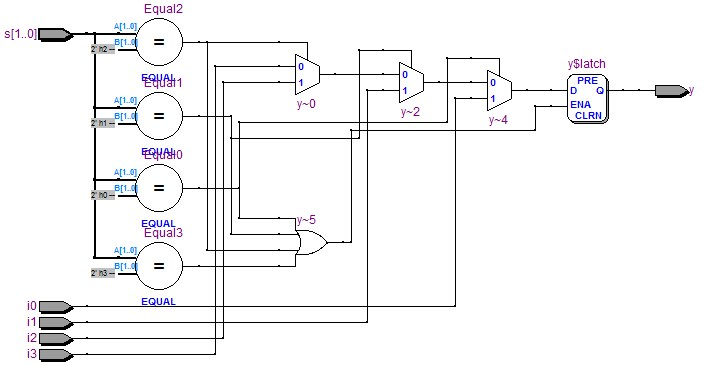
\includegraphics[width=0.8\textwidth]{ifEx}
	\caption{Multiplexer using if statement, Listing \ref{vhdl:ifEx}}
	\label{fig:ifEx}
\end{figure}
\begin{figure}
	\centering
	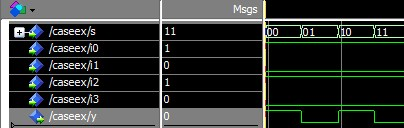
\includegraphics[scale=1]{ifExWave}
	\caption{Waveforms of Listing \ref{vhdl:ifEx} and \ref{vhdl:caseEx}}
	\label{fig:ifExWave}
\end{figure}




\section{Case statement}
Case statement is shown in lines 17-28 of Listing \ref{vhdl:caseEx}. `s' is defined in case statement at line 17; whose value is checked using `when' keyword at lines 18 and 20 etc. The value of `y' depends on the value of `s' e.g. if `s' is ``01'', then line 20 will be true, hence value of `i1' will be assigned to `y'. 

\begin{noNumBox}
	Note that the `multiplexer design' in Fig. \ref{fig:caseEx} (generated by case in Listing \ref{vhdl:caseEx}) is exactly same as the design in Fig. \ref{fig:multiplexerVhdl} (generated by with-select in Listing \ref{vhdl:multiplexerVhdl}). 
\end{noNumBox}


\lstinputlisting[
language = Vhdl,
caption    = {Multiplexer using case statement},
label      = {vhdl:caseEx}
]{caseEx.vhd}
\begin{figure}
	\centering
	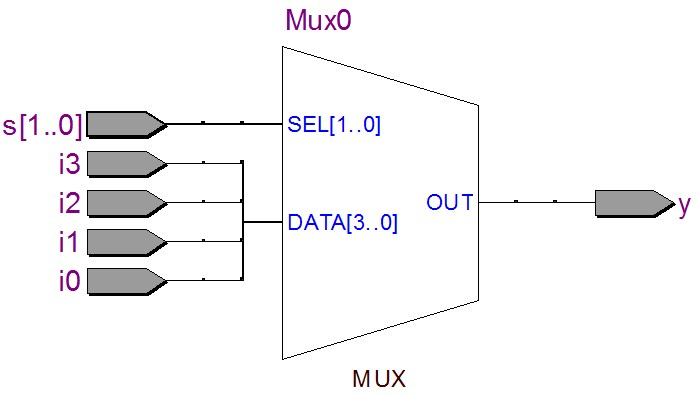
\includegraphics[scale=0.4]{caseEx}
	\caption{Multiplexer using case statement, Listing \ref{vhdl:caseEx}}
	\label{fig:caseEx}
\end{figure}


\section{Problem with Loops}

VHDL provides two loop statements i.e. `for' loop and `while' loop'. These loops are very different from software loops. Suppose `for i = 1 to N' is a loop', then, in software `i' will be assigned one value at time i.e. first i=1, then next cycle i=2 and so on. Whereas in VHDL, N logic will be implement for this loop, which will execute in parallel. Also, in software, `N' cycles are required to complete the loop, whereas in VHDL the loop will execute in one cycle. 
\begin{noNumBox}
	As loops implement the design-units multiple times, therefore design may become large and sometimes can not be synthesized as well. If we do not want to execute everything in one cycle (which is almost always the case), then loops can be replaced by `case' statements and `conditional' statements as shown in section \ref{sec:ifLoop}. Further, due to these reasons, we do not use loops in the design, and hence these are not discussed in the tutorial.
\end{noNumBox}   

\section{Loop using `if' statement}\label{sec:ifLoop}
In Listing \ref{vhdl:ifLoop}, a loop is created using `if' statement, which counts the number upto input `x'. 

\begin{explanation}[Listing \ref{vhdl:ifLoop}]
	In the listing, two `process' blocks are used i.e. at lines 20 and 31. The process at line 20 checks whether the signal `count' value is `less or equal' to input x (line 22), and sets the currentState to `continueState'; otherwise if count is greater than the input x, then currentState is set to `stopState'.
	
	Then next process statement (line 31), increase the `count' by 1, if currentState is `continueState'; otherwise count is set to 0 for stopState. Finally count is displayed at the output through line 39. In this way, we can implement the loops using process statements. 
	
	Fig. \ref{fig:ifLoop} shows the loop generated by the listing with generic value N=1. Further,  Fig. \ref{fig:ifLoopWave} shows the count-waveforms generated by the listing with generic value N = 3.
\end{explanation}

\lstinputlisting[
language = Vhdl,
caption    = {Loop using `if' statement},
label      = {vhdl:ifLoop}
]{ifLoop.vhd}
\begin{figure}[!h]
	\centering
	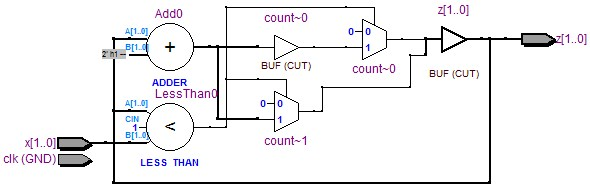
\includegraphics[width=\textwidth]{ifLoop}
	\caption{Loop using `if' statement, Listing \ref{vhdl:ifLoop} with N = 1}
	\label{fig:ifLoop}
\end{figure}

\begin{figure}[!h]
	\centering
	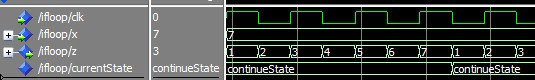
\includegraphics[width=\textwidth]{ifLoopWave}
	\caption{Loop using `if' statement, Listing \ref{vhdl:ifLoop} with N = 3}
	\label{fig:ifLoopWave}
\end{figure}

\begin{noNumBox}
	Sensitivity list of the process block should be implemented carefully. For example, if we add `count' in the sensitivity list at line 31 of Listing  \ref{vhdl:ifLoop}, then the process block will execute infinite times. This will occur because the process block execute whenever there is any event in the signals in the sensitivity list; therefore any change in `count' will execute the block, and then this block will change the `count' value through line 34. Since `count' value is changed, therefore process block will execute again, and the loop will never exit.  
\end{noNumBox}

\section{Conclusion}
In this chapter, various statements of behavioral modeling styles are discussed. Also, we saw the relationship between the designs generated by behavior modeling and dataflow modeling. Further, problem with loops are discussed and finally loop is implemented using `if' statement. 